\section{Drone and Base Station Sample Implementation}
In order to demonstrate the capabilities of the octoDrone product, both through the simulation and physical drones, a sample set of code was written. This demonstrative drone network uses heat sensors on the drones to collect temperature data across a predefined area. This does, of course, draw an immediate link with the forest fires prevalent in California. Once the 'normal' temperatures for an area are monitored, it could be extended such that any unexpected change to this temperature might mean there is the beginnings of a fire. Once alerted, wardens could confirm or refute this premise using cameras on the drone. This chapter covers the implementation of the demonstration code and physical routing algorithms used.

\subsection{The Base Station}
In this network, as expected, the base station will perform the task of disseminating work between the drones. In addition to this, it will be responsible for collating the data from the drones as it is being collected. Firstly, however, the base station broadcasts its address to everything nearby so that the drones know who to send temperature data to. This avoids flooding the channels with broadcasts to everything. Following this, the base station waits for a set amount of time during which it will receive the addresses of the drones in the network. These addresses are then stored as a vector on the base station.

Once this has been done, the base station determines which sections of the defined area will be allocated to each drone. This is done simply by splitting the area 1-dimensionally along the x-direction, where each drone is responsible for all points in the y-direction as shown in figure \ref{fig:area_dissemination}. The base station then waits messages from the drones containing temperature information.

\begin{figure}[h!]
\centering
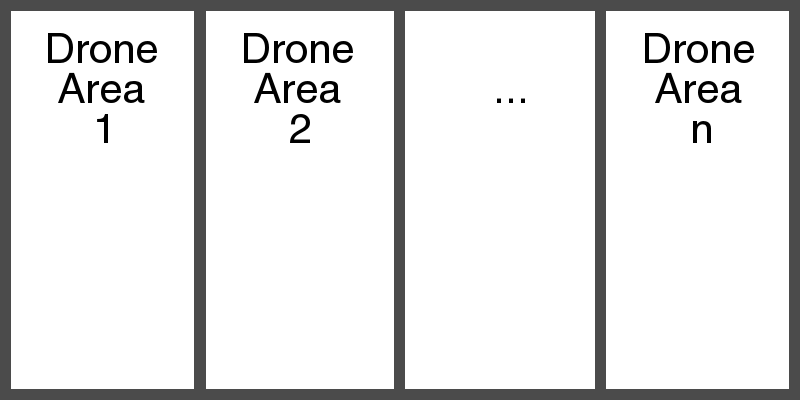
\includegraphics[width=15cm]{DroneAreas}
\caption{Dissemination of the area to drones.}
\label{fig:area_dissemination}
\end{figure}

\subsection{The Drones}
Similarly to the base station, the first thing the drones do is broadcast their address to everything around, followed by waiting to receive the address of the base station. Before the drones then do anything, they wait for the areas that they are to collect data on. Once this has been received, the drones systematically travel to each allocated point in space, measuring the temperature and moving onto the next. The physical routing techniques used for this are described in section \ref{sec:physicalrouting_collsionavoidance}.

Each time a drone collects data from a point in the area, it sends that data back to the base station immediately, meaning the base station receives many small messages each containing a single data point. This was done for two reasons. Firstly, the base station can spread the work of combining the data over the course of the system execution. Secondly, this means that if one of the drones fails, then its previous work is not lost.

\subsection{Handling Messages}

The reliable delivery of messages between the drones and base station are handled by the communication module. However, the implementation of a given system must specify how the messages are acting upon and how they are managed. For this implementation, both the drone and base station listen for messages during their program loops. When a messages is received it is then 'interpreted' by entering into a separate function that deals with all possible actions that might need to be done regarding a messages. For example, A drone might receive a message informing it of the base station's IP address. The table in figure \ref{tbl:messages_drone} shows the messages that the drone understands on top of those implemented by the base simulation software. Figure \ref{tbl:messages_basestation} shows the same for the base station.

\begin{figure}
\begin{tabular}{c|l|l}
Label & Data & Action to Take \\
NEWAREA	& Four values making a 2D rectangle	& Set this area as the new area to collect data over. Call the function to split this into points. \\
BASEIP & An IP Address & Record this IP address as the base station's IP address. \\
DRONEIP	& An IP Address	& Record this IP address in the list of drone IP addresses. \\
LOC	& The current location, angle, speed and routing priority of another drone & Perform collision avoidance. \\
\end{tabular}
\caption{Table showing the messages a drone understands}
\label{tbl:messages_drone}
\end{figure}

\begin{figure}
\begin{tabular}{c|l|l}
Label	& Data							& Action to Take	\\
DRONEIP	& An IP Address					& Record this IP address in the list of drone IP addresses. \\
DATUM	& A point location and value	& This is a data value from a drone so record it.
\end{tabular}
\caption{Table showing the messages the base station understands}
\label{tbl:messages_basestation}
\end{figure}

\subsection{What Does this Demonstrate?}
This sample application demonstrates that it is very much possible for a working drone network to be built using the simulation. It shows the drones working autonomously and separate from each other, as well as a base station performing a similar task as would be expected in a real-world application. While this system only provides simple functionality, it demonstrates the possibility for a wide array of applications using fault tolerance, efficient communication, and robust physical routing.

\subsection{Area Representation}

As described in the physical routing section of the design, the drone's understanding of the world is in 3-dimensional Cartesian coordinates. However, for this implementation, the drone does not concern itself with the potential for obstacles in the area it is measuring as it is assumed to be completely open. From this, this means there is no need to store a representation of the 'map' on the drone, but only of the points that the drone should be travelling to and measuring.

When the drone receives the area it is to sense over, it is in the form of four values corresponding to the x-min, y-min, x-max, and y-max denoting a 2-dimensional plane. Using the sensing radius of the drone's sensing equipment, passed in as arguments to the drone when it is started, the drone determines how many measurements it will need to perform in order to cover the whole area. These points are then stored in a C++ queue so that the elements can be accessed in a strict order. The ordering walks up and down the area so that the drone has to travel the smallest distance between points. The queue is efficient and easy to iteratively add to as opposed to a vector.

\subsection{Collision Avoidance}
\label{sec:physicalrouting_collsionavoidance}

The overall physical routing technique used for collision avoidance was described in the physical routing design section. It was implemented as described there, with both drones calculating if a collision would occur and, if one would, one flying higher than the other so that the collision is avoided.

In order to detect if a collision might occur, then each drone, when sending broadcasting its location to all other drones around, also includes its current position, facing, speed, and priority. Each drone sends this broadcast with the frequency meaning that the interval between broadcasts can be used as the maximum time we need to check for collisions in. From this information, the maximum change in the x direction for this timestep is given by,
\begin{verbatim}
	dx = t * 2 * s * sin(\theta)
\end{verbatim}
and the maximum change in the y direction is given by,
\begin{verbatim}
	dy = t * 2 * s * cos(\theta)
\end{verbatim}
where t is the broadcast interval, s is the speed of the drone, and $\theta$ is the current facing of the drone.

\begin{figure}[h!]
\centering
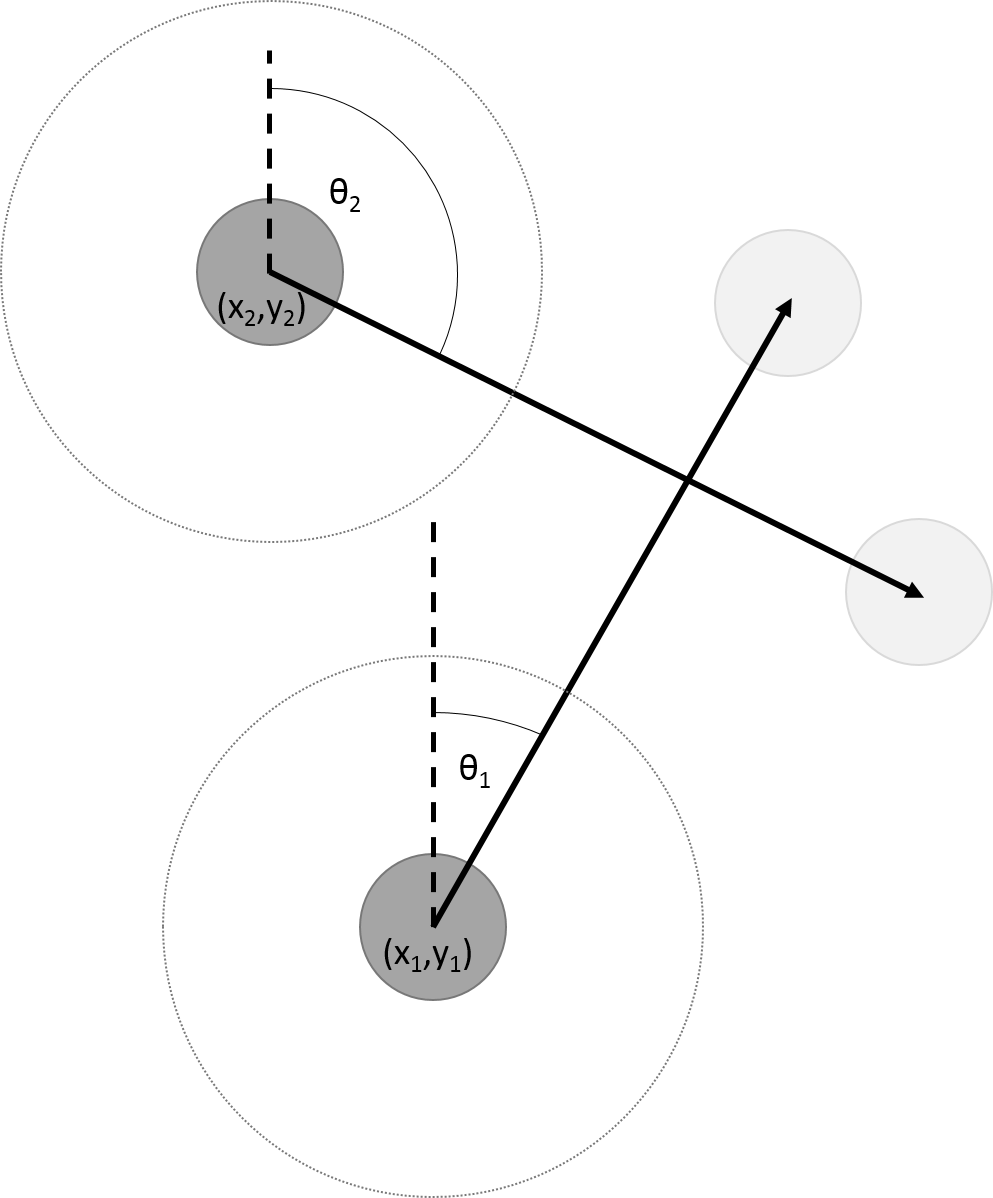
\includegraphics[width=15cm]{DroneFlight}
\caption{Two drones and their projected paths with $\theta$ angles shown.}
\label{fig:drone_flight}
\end{figure}

Unfortunately, this alone leaves the issue presented if the drones are moving too fast and will not collide at the end of their movement, but rather at single point during their movement. While it is possible to extrapolate back from the collision to find the exact point of collision, for this it is not necessary to know exactly where and when the drones would collide, only that they will so it can be avoided. Because of this, the algorithm then checks for a collision another four times along the path of the drones.

It is worth noting that this whole calculation is only done by the drone with the lower priority as only it will need to know if it should be getting out of the way. This means only the half the computation is required across the drones in total.